\documentclass[10pt,letterpaper]{article}
\RequirePackage{amsthm,amssymb,amsmath,graphicx}
\RequirePackage[top=2cm, bottom=2cm, left=2.5cm, right=3cm]{geometry}
\usepackage{caption}
\usepackage{subcaption}
\usepackage[pagebackref=false,colorlinks,linkcolor=black,citecolor=magenta]{hyperref}
\RequirePackage{MnSymbol}
\newcommand{\eqn}[2]{
\begin{equation}
\begin{split}
#1
\label{#2}
\end{split}
\end{equation}
}
%%%%%%%%%%%%%

%       \eqn{
%       x=x^2
%       }{label}

%%%%%%%%%%%%%
\newcommand{\feqn}[2]{
\begin{tcolorbox}[width=7in, colback=white]
\begin{equation}
\begin{split}
#1
\label{#2}
\end{split}
\end{equation}
\end{tcolorbox}
}
%%%%%%%%%%%%%%%
\newcommand{\hl}{
\begin{center}
\line(1,0){450}
\end{center}}
\setlength{\parindent}{0pt}
\newcommand{\nl}{\newline\newline}
\newcommand{\pic}[1]{
\begin{center}
\includegraphics[width=130mm]{#1}
\end{center}
}
%\settextfont{B Nazanin}
\usepackage{lipsum}
\begin{document}
\Large
\begin{center}
The assignment \#7 of the \textbf{ComNet} course
\hl
\end{center}
Q1) 

Consider the following network topology:
\begin{center}
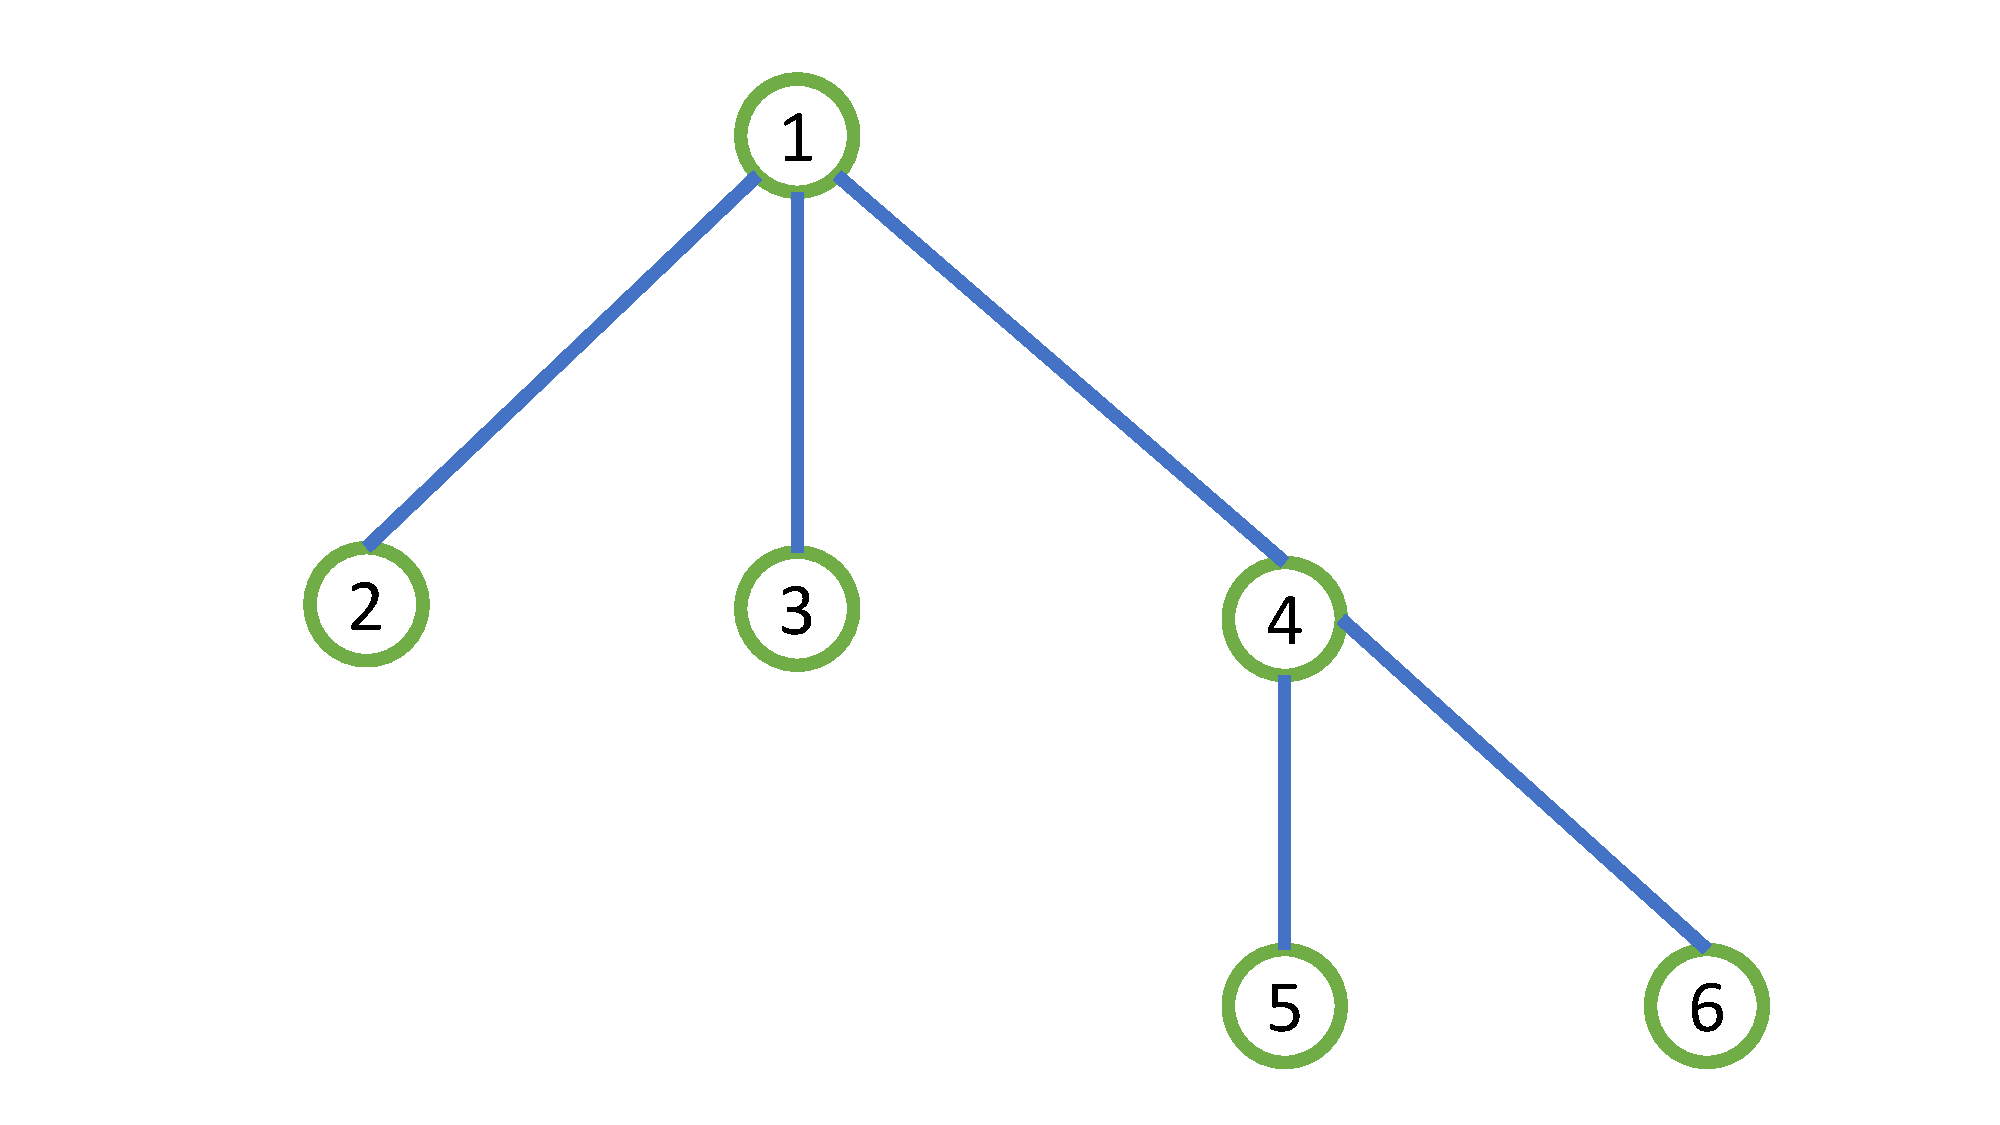
\includegraphics[width=120mm]{Q1_HW7}
\end{center}
How much data is transported over all the links in total, assuming that the node $1$ wants to broadcast a packet of length 1Mbytes if

a. uncontrolled flooding is used

b. controlled flooding is used with \textbf{R}everse \textbf{P}ath \textbf{F}orwarding (RPF)

c. minimum spanning tree is used with center point approach (also, show your work on building such a tree where the center node is $2$. Obviously, the answer may not be unique)

?
\newline
\newline
Q2)

a.) Are IGMP messages layer 3 datagrams? Explain.

b) How does a router find out whether or not a host has left a multicast group, asuming that the \texttt{leave\_group} IGMP message is not used at all?
\newline
\newline
Q3) Consider a network in which all nodes are connected to three other nodes. In a single time step, a node can receive all transmitted broadcast packets from its neighbors, duplicate the packets, and send them to all of its neighbors (except to the node that sent a given packet). At the next time step, neighboring nodes can receive, duplicate, and forward these packets, and so on. Suppose that uncontrolled flooding is used to provide broadcast in such a network. At time step t, how many copies of the broadcast packet will be transmitted, assuming that during time step 1, a single broadcast packet is transmitted by the source node to its three neighbors.
\newline
\newline
Q4)

Assume a 3-bit data is being encoded with the 3-bit generator $G=111$. The constructed data $D\cdot 2^r+R$ is then sent on the channel which is divisible by $G$. Based on the discription of CRC, the receiver checks whether the arrived data is divisible by $G$. If not, an error is declared. The channel reverts a single bit with a probability of $p$.

a) what is the probability that an error occurs but does not become declared? Calculate it for $p=0.01$. (Hint: you can use the MATLAB \texttt{dec2bin()} function to calculate the binary expansion of a positive integer)

b) assume that we simply use a single-bit parity check instead of CRC, i.e. we sum up all the binary digits of the original $3$-bit data and add it up at the end of the data before transmission. The receiver then simply adds up all four bits of the arriving data. An error is declared only if the sum is $1$. What is the probability that an error occurs but does not become declared? Calculate it for $p=0.01$.

c) why is the probability of error miss-detection of one of the parts ``a'' or ``b'' significantly less than the other one? What was the trade-off?
\end{document}